\begin{center}
\end{center}
\begin{center}
\end{center}



\tikzset{every picture/.style={line width=0.75pt}} %set default line width to 0.75pt        

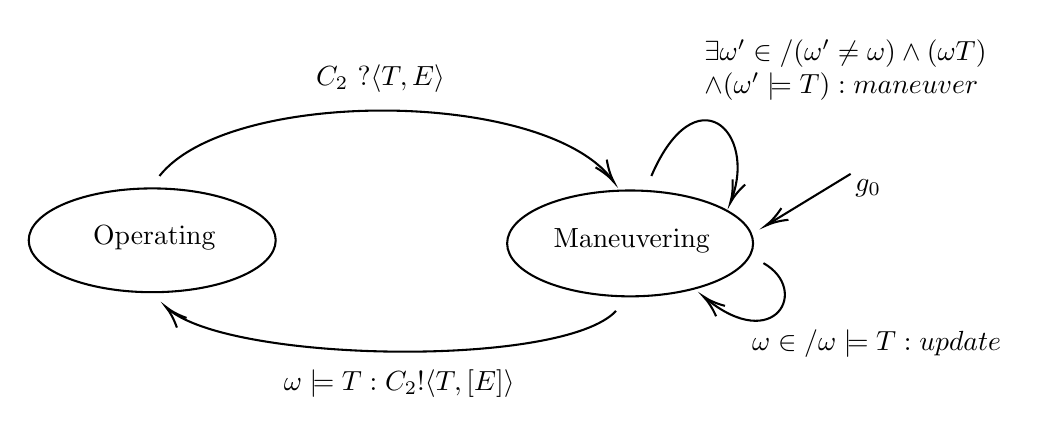
\begin{tikzpicture}[x=0.75pt,y=0.75pt,yscale=-1,xscale=1]
%uncomment if require: \path (0,215); %set diagram left start at 0, and has height of 215

%Curve Lines [id:da9480858267519683] 
\draw    (135.5,88) .. controls (169.16,45.43) and (320.43,45.98) .. (353.53,89.66) ;
\draw [shift={(354.5,91)}, rotate = 235.44] [color={rgb, 255:red, 0; green, 0; blue, 0 }  ][line width=0.75]    (10.93,-3.29) .. controls (6.95,-1.4) and (3.31,-0.3) .. (0,0) .. controls (3.31,0.3) and (6.95,1.4) .. (10.93,3.29)   ;

%Shape: Ellipse [id:dp6594609066072359] 
\draw   (72.5,119) .. controls (72.5,105.19) and (99.14,94) .. (132,94) .. controls (164.86,94) and (191.5,105.19) .. (191.5,119) .. controls (191.5,132.81) and (164.86,144) .. (132,144) .. controls (99.14,144) and (72.5,132.81) .. (72.5,119) -- cycle ;
%Shape: Ellipse [id:dp873836537729809] 
\draw   (303,120.5) .. controls (303,106.42) and (329.53,95) .. (362.25,95) .. controls (394.97,95) and (421.5,106.42) .. (421.5,120.5) .. controls (421.5,134.58) and (394.97,146) .. (362.25,146) .. controls (329.53,146) and (303,134.58) .. (303,120.5) -- cycle ;
%Curve Lines [id:da3135064064897334] 
\draw    (355.5,153) .. controls (329.89,180.58) and (170.39,178.08) .. (139.81,152.2) ;
\draw [shift={(138.5,151)}, rotate = 405] [color={rgb, 255:red, 0; green, 0; blue, 0 }  ][line width=0.75]    (10.93,-3.29) .. controls (6.95,-1.4) and (3.31,-0.3) .. (0,0) .. controls (3.31,0.3) and (6.95,1.4) .. (10.93,3.29)   ;

%Curve Lines [id:da21020703050779688] 
\draw    (372.5,88) .. controls (393.68,38.75) and (423.59,66.15) .. (411.1,99.47) ;
\draw [shift={(410.5,101)}, rotate = 292.38] [color={rgb, 255:red, 0; green, 0; blue, 0 }  ][line width=0.75]    (10.93,-3.29) .. controls (6.95,-1.4) and (3.31,-0.3) .. (0,0) .. controls (3.31,0.3) and (6.95,1.4) .. (10.93,3.29)   ;

%Curve Lines [id:da14662580418826565] 
\draw    (426.5,130) .. controls (449.16,142.81) and (432.03,174.04) .. (399.02,147.26) ;
\draw [shift={(397.5,146)}, rotate = 400.46000000000004] [color={rgb, 255:red, 0; green, 0; blue, 0 }  ][line width=0.75]    (10.93,-3.29) .. controls (6.95,-1.4) and (3.31,-0.3) .. (0,0) .. controls (3.31,0.3) and (6.95,1.4) .. (10.93,3.29)   ;

%Straight Lines [id:da37650774099478246] 
\draw    (468.5,87) -- (429.21,110.96) ;
\draw [shift={(427.5,112)}, rotate = 328.63] [color={rgb, 255:red, 0; green, 0; blue, 0 }  ][line width=0.75]    (10.93,-3.29) .. controls (6.95,-1.4) and (3.31,-0.3) .. (0,0) .. controls (3.31,0.3) and (6.95,1.4) .. (10.93,3.29)   ;


% Text Node
\draw (133,118) node  [align=left] {Operating};
% Text Node
\draw (363,119) node  [align=left] {Maneuvering};
% Text Node
\draw (242,41) node   {$C_{2} \ ?\langle T,E\rangle $};
% Text Node
\draw (251,188) node   {$\omega \models T:C_{2} !\langle T,[ E] \rangle $};
% Text Node
\draw (477,94) node   {$g_{0}$};
% Text Node
\draw (481,169) node   {$\nexists \omega \in \si{\ohm}/\omega \models T:update$};
% Text Node
\draw (466,37) node   {$ \begin{array}{l}
\exists \omega '\in \si{\ohm}/( \omega '\neq \omega ) \land ( \omega \nvDash T)\\
\land ( \omega '\models T) :maneuver
\end{array}$};


\end{tikzpicture}